\chapter{Spiking Neural Networks~(SNNs)}
\label{cha:bkg}
This chapter aims to introduce fundamental concepts of spiking neurons, which are basic processing units of SNNs, and all the proposed work in the thesis will be built on such units.
Hence, we will start from the elementary neuroscience notions in Section~\ref{sec:neuron_basic} to give a general impression of a spiking neuron and neural signals propagated among network of neurons.
These neural signalling dynamics can be abstracted and simplified by mathematical models, for example leaky integrate-and-fire~(LIF) model, which will be a popular neural model used in our research.
Thus, Section~\ref{sec:spike} will present neural dynamic modelling by taking the example of LIF neurons, and a modelled biological-plausible learning rule.
To operate networks of spiking neurons, in Section~\ref{sec:snn_sim} we will introduce the simulators both in software and hardware, including neuromrophic systems.


%The so-called third generation of neural networks~\cite{maass1997networks} introduces a different set of functions and parameters to model neurons;
%%these both model biological neurons more precisely~\cite{hodgkin1952quantitative} and increase the computational power of networks of neurons if compared to classical sigmoidal units.
%it models the biological neurons more precisely and increases the computational power of neural networks when compared to the classical sigmoid functions.
%Such networks rely on the propagation of an all-or-none signal, the action potential, which asynchronously carries information to its connected units by means of its timing.
\section{Neural System Basics}
\label{sec:neuron_basic}
Over the past hundred years, biological research has accumulated an enormous amount of detailed knowledge about the structure and function of the brain.
The elementary processing units in the central nervous system are neurons, which are connected to each other in an intricate pattern.
In reality, cortical neurons and their connections are packed into a dense network with more than $10^{4}$ cell bodies and several kilometers of ‘wires’ per cubic millimeter. Across areas of the brain the wiring pattern may look different.
In all areas, however, neurons of different sizes and shapes form the basic elements.

	\begin{figure}[bt]
		\centering
		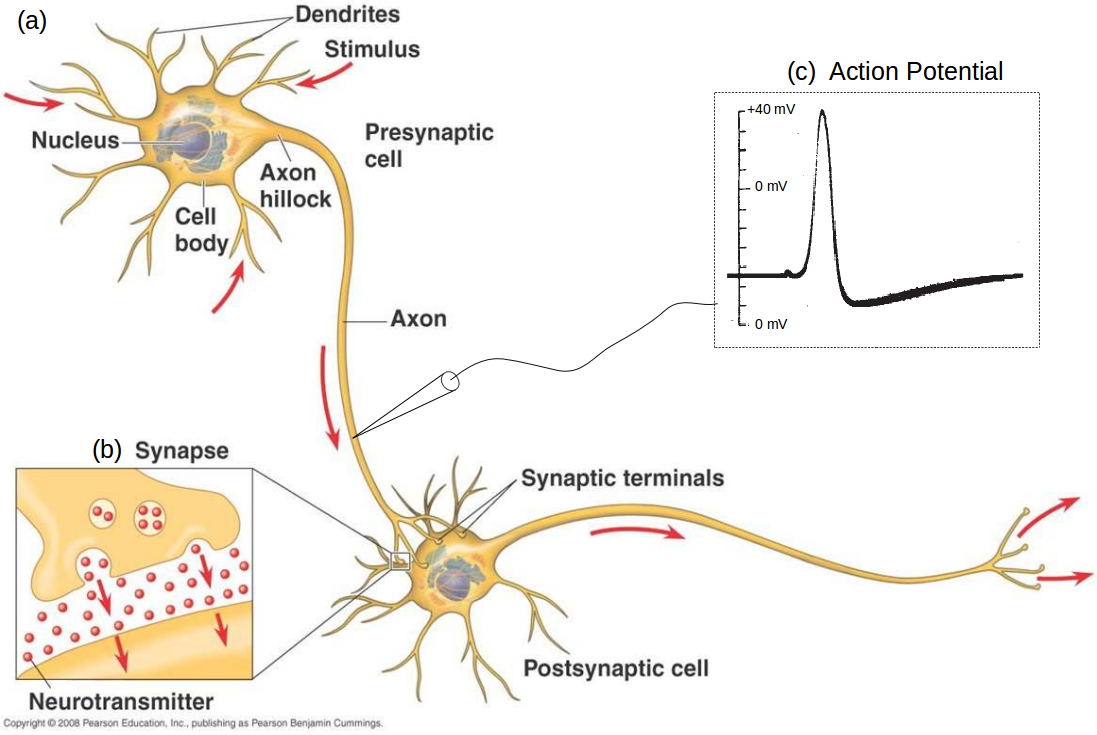
\includegraphics[width=0.98\textwidth]{pics_snn/neuron2.png}
		\caption{Two neurons connected by synapses. 
			A neuron mainly is composed of three functional parts: dendrites, the soma, and the axon. (a) A Presynaptic cell connects to its postsynaptic cell through synapses~\cite{reece2011campbell}, see (b)~\cite{reece2011campbell}, and the neural signal, action potential see (c)~\cite{hodgkin1939action}, propagates along the red arrows. }
		\label{Fig:neuron_basic}
	\end{figure}

\subsection{Biological Neural Components}
%\subsubsection{Neurons}
What composes a spiking neuron?

A typical neuron can be divided into three functionally distinct parts, called dendrites, soma, and axon; see Fig. 1.2. Roughly speaking, the dendrites play the role of the ‘input device’ that collects signals from other neurons and transmits them to the soma. The soma is the ‘central processing unit’ that performs an important non-linear processing step: If the total input arriving at the soma exceeds a certain threshold, then an output signal is generated. The output signal is taken over by the ‘output device’, the axon, which delivers the signal to other neurons.

The junction between two neurons is called a synapse. Let us suppose that a neuron sends a signal across a synapse. It is common to refer to the sending neuron as the presynaptic cell and to the receiving neuron as the postsynaptic cell. A single neuron in vertebrate cortex often connects to more than $10^{4}$ postsynaptic neurons. Many of its axonal branches end in the direct neighborhood of the neuron, but the axon can also stretch over several centimeters so as to reach neurons in other areas of the brain.

%Spiking neuron models can be divided into two major categories \cite{gernstbook} based on their level of abstraction: The conductance models and the threshold models.
%The conductance models simulate a lower level on the ion channels, while the threshold models represent a higher level of neuron abstraction where the threshold voltage is fixed and the neuron fires once the membrane potential reaches it.
%
%In general, Conductance-Based models have been derived from the Nobel prize winners (1963) Hodgkin and Huxley, based on the experiments that they performed on the giant axon squid \cite{hhmodel}.
%Spikes arriving at a LIF neuron cause a temporary flow of current into (excitatory synapse) or out of (inhibitory synapse) the neuron, modelling the behaviour of synapses in biological neurons.
%The LIF neuron sums up this current over time, accumulating charge which gradually leaks away.
%If the membrane potential in the neuron reaches a certain threshold, it produces a spike and its charge is reset.
%LIF neurons have been extensively used in large spiking neural networks \cite{Delorme1999989} because of their ease of implementation and the low computational cost.

%\subsubsection{Spikes}

%\subsubsection{Synapses}

\subsection{Neuronal Signals}

What is the signal transited among neurons?
and what are the codes.

The neuronal signals consist of short electrical pulses and can be observed by placing a fine electrode either on the soma or close to the soma or axon of a neuron; see Fig. 1.2. The pulses, so-called action potentials or spikes, have an amplitude of about 100 mV and typically a duration of 1-2 ms. The form of the pulse does not change as the action potential propagates along the axon. A chain of action potentials emitted by a single neuron is called a spike train – a sequence of stereotyped events which occur at regular or irregular intervals; see Fig. 1.3. Since isolated spikes of a given neuron look alike, the form of the action potential does not carry any information. Rather, it is the number and the timing of spikes which matter. The action potential is the elementary unit of signal transmission.

Action potentials in a spike train are usually well separated. Even with very strong input, it is impossible to excite a second spike during or immediately after a first one. The minimal distance between two spikes defines the absolute refractory period of the neuron. The absolute refractory period is followed by a phase of relative refractoriness where it is difficult, but not impossible to excite an action potential.

%Code:https://www.slideshare.net/ieee_cis_cyprus/jennie-si
The rate coding model of neuronal firing communication states that as the intensity of a stimulus increases, the frequency or rate of action potentials, or ``spike firing'', increases. Rate coding is sometimes called frequency coding.
An example of V1 simple cell responding to its visual stimuli is shown in Figure~\ref{Fig:v1}.

\begin{figure}[bt]
	\centering
	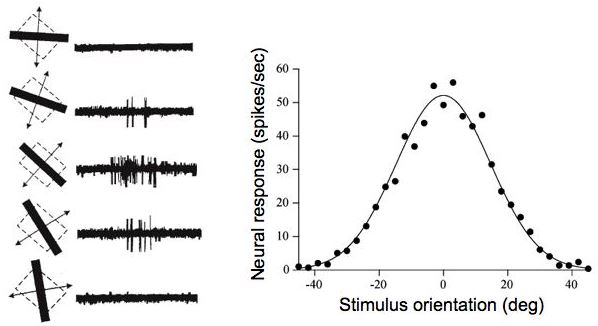
\includegraphics[width=0.8\textwidth]{pics_snn/v1.jpg}
	\caption{Example of rate coding: cat V1~\cite{hubel1962receptive}.}
	\label{Fig:v1}
\end{figure}

For very brief stimuli, a neuron's maximum firing rate may not be fast enough to produce more than a single spike. Due to the density of information about the abbreviated stimulus contained in this single spike, it would seem that the timing of the spike itself would have to convey more information than simply the average frequency of action potentials over a given period of time. This temporal code is especially important for sound localization, which occurs within the brain on the order of milliseconds. The spikes generated phase-locked to input sound (sine wave) by an inner ear cell is shown in Figure~\ref{Fig:audio_fibre}. The brain must obtain a large quantity of information based on a relatively short neural response. Additionally, if low firing rates on the order of ten spikes per second must be distinguished from arbitrarily close rate coding for different stimuli, then a neuron trying to discriminate these two stimuli may need to wait for a second or more to accumulate enough information. This is not consistent with numerous organisms which are able to discriminate between stimuli in the time frame of milliseconds, suggesting that a rate code is not the only model at work.


\begin{figure}[bt]
	\centering
	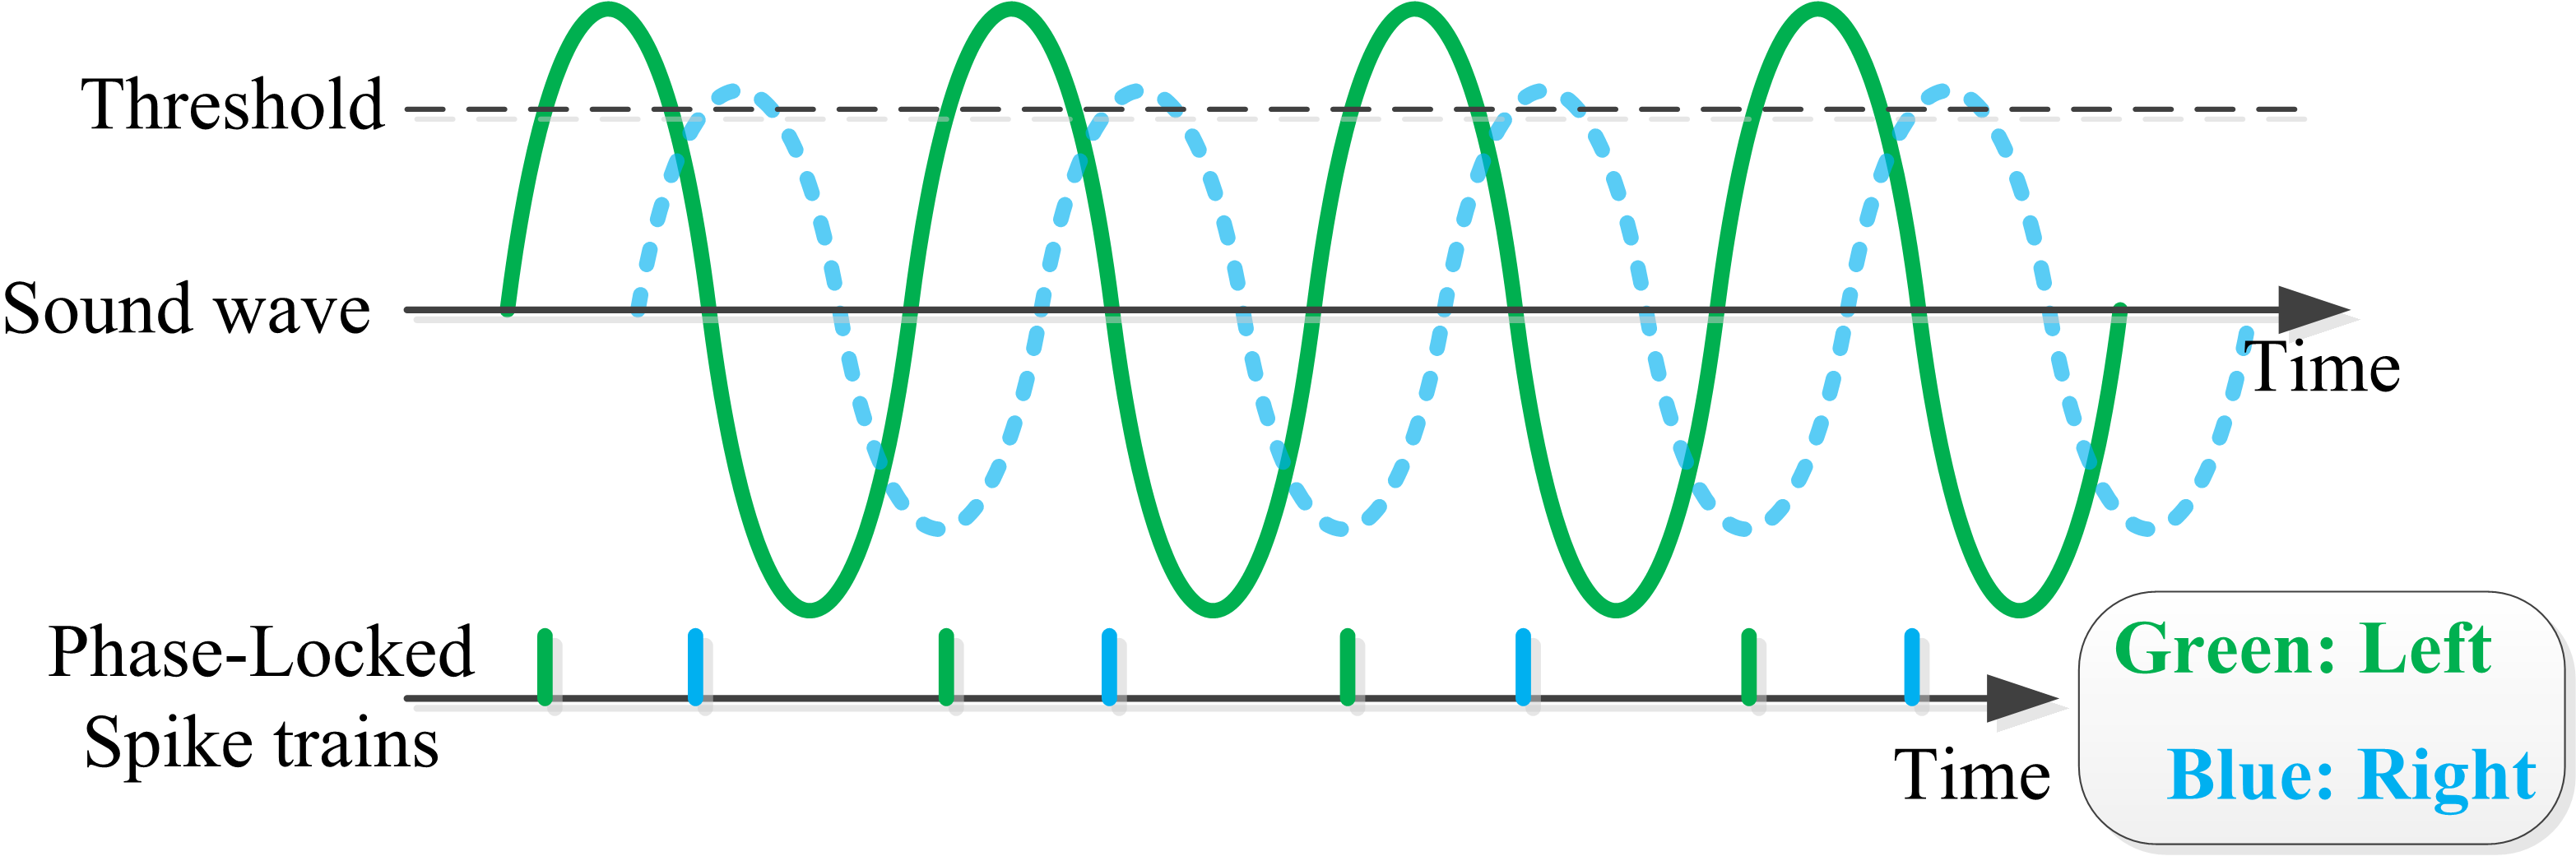
\includegraphics[width=0.8\textwidth]{pics_snn/phaselocking.png}
	\caption{Example of temporal coding: auditory fibre~\cite{liu2013modeling}.}
	\label{Fig:audio_fibre}
\end{figure}

\subsection{Signal Transmission}
How these signals are propagated? 

The site where the axon of a presynaptic neuron makes contact with the dendrite (or soma) of a postsynaptic cell is the synapse. The most common type of synapse in the vertebrate brain is a chemical synapse. At a chemical synapse, the axon terminal comes very close to the postsynaptic neuron, leaving only a tiny gap between pre- and postsynaptic cell membrane. This is called the synaptic cleft. When an action potential arrives at a synapse, it triggers a complex chain of bio-chemical processing steps that lead to a release of neurotransmitter from the presynaptic terminal into the synaptic cleft. As soon as transmitter molecules have reached the postsynaptic side, they will be detected by specialized receptors in the postsynaptic cell membrane and lead (either directly or via a biochemical signaling chain) to an opening of specific channels causing ions from the extracellular fluid to flow into the cell. The ion influx, in turn, changes the membrane potential at the postsynaptic site so that, in the end, the chemical signal is translated into an electrical response. The voltage response of the postsynaptic neuron to a presynaptic spike is called the postsynaptic potential.




\section{Modelling Spiking Neurons}
\label{sec:spike}
\subsection{Neural Dynamics}
\subsubsection{Membrane Potential}
The effect of a spike on the postsynaptic neuron can be recorded with an intracellular electrode which measures the potential difference $V(t)$ between the interior of the cell and its surroundings. This potential difference is called the membrane potential. Without any input, the neuron is at rest corresponding to a constant membrane potential $V_{rest}$. After the arrival of a spike, the potential changes and finally decays back to the resting potential, Figure~\ref{Fig:neural_dynamics}(a).
If the change is positive, the synapse is said to be excitatory. If the change is negative, the synapse is inhibitory.

At rest, the cell membrane has already a strongly negative polarization of about –65 mV. An input at an excitatory synapse reduces the negative polarization of the membrane and is therefore called depolarizing. An input that increases the negative polarization of the membrane even further is called hyperpolarizing.


\begin{figure}[tbh!]
	\centering
	\begin{subfigure}[t]{0.7\textwidth}
		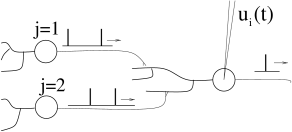
\includegraphics[width=\textwidth]{pics_snn/x10.png}
		\caption{An electrode measures the \textbf{membrane potential} of a postsynaptic neuron which connected by two presynaptic neurons.}
	\end{subfigure}\\
	\begin{subfigure}[t]{0.6\textwidth}
		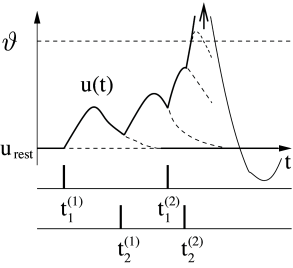
\includegraphics[width=\textwidth]{pics_snn/x11.png}
		\caption{\textbf{Postsynaptic potential (PSP)} generated by spikes of its presynaptic neurons adds up to its \textbf{membrane potential} change. }
	\end{subfigure}
	\caption{A postsynaptic neuron $i$ receives input from two presynaptic neurons $j=1,2$.}
	\label{Fig:neural_dynamics}
\end{figure}

%\begin{figure}[bt]
%	\centering
%	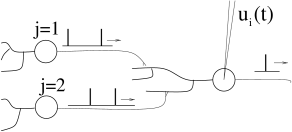
\includegraphics[width=0.6\textwidth]{pics_snn/x10.png}
%	\caption{An electrode measures the membrane potential of a postsynpatic neuron~\cite{gerstner2014neuronal}.}
%	\label{Fig:mem_potential}
%\end{figure}
%
\subsubsection{Postsynaptic Potential}
Let us formalize the above observation. We study the time course $V_i(t)$ of the membrane potential of neuron $i$. 
Before the input spike has arrived, we have $V_i(t) = V_{rest}$. At t=0 t=0 the presynaptic neuron $j$ fires its first spike. For $t>0$, we see at the electrode a response of neuron $i$:
\begin{equation}
PSP_{ij}(t) = V_i(t) - V_{rest}~~.
\end{equation}
If the voltage difference is positive (negative) we have an excitatory (inhibitory) postsynaptic potential or short EPSP (IPSP). In Figure~\ref{Fig:neural_dynamics}(b) we have sketched four EPSPs caused by the arrival of spikes from presynaptic neurons at excitatory synapses of neuron $i$.
As long as there are only few input spikes, the total change of the potential is approximately the sum of the individual PSPs:
\begin{equation}
V_i(t) = \sum_j\sum_f PSP_{ij}(t-t_j^{(f)}) + V_{rest}~~.
\end{equation}

\subsubsection{Membrane Threshold}

As soon as the membrane potential reaches a critical value $V_{thresh}$, its trajectory shows a behaviour that is quite different from a simple summation of PSPs: The membrane potential exhibits a pulse-like excursion with an amplitude of about 100 mV. This short voltage pulse will propagate along the axon of neuron $i$ to the synapses with other neurons. After the pulse the membrane potential does not directly return to the resting potential, but passes, for many neuron types, through a phase of hyperpolarization below the resting value. This hyperpolarization is called ‘spike-afterpotential’.

Single EPSPs have amplitudes in the range of one millivolt. The critical value for spike initiation is about 20 to 30 mV above the resting potential. In most neurons, four spikes – as shown schematically in Fig. 1.5C – are thus not sufficient to trigger an action potential. Instead, about 20-50 presynaptic spikes have to arrive within a short time window to trigger a postsynaptic action potential.
%\begin{figure}[bt]
%	\centering
%	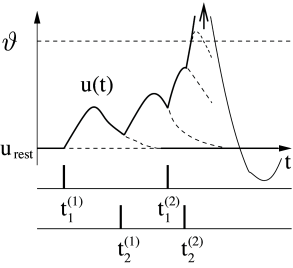
\includegraphics[width=0.6\textwidth]{pics_snn/x11.png}
%	\caption{A postsynpatic neuron receives input from two neurons which fires at time $t$~\cite{gerstner2014neuronal}.}
%	\label{Fig:psp}
%\end{figure}

\subsection{Neural Models}
To model a spiking neuron is to mathematically formalise its neural dynamics of PSP, and the reset of its membrane potential after an action potential.
% and the hyperpolarization below the resting potential.

\subsubsection{Leaky Integrate-and-Fire}
In order to analyze the circuit, we use the law of current conservation and split the driving current into two components,
%
%I(t)=IR+IC
%I(t)=I_{R}+I_{C}
%(1.3)
%The first component is the resistive current IR I_{R} which passes through the linear resistor R R. It can be calculated from Ohm’s law as IR=uR/R I_{R}=u_{R}/R where uR=u−urest u_{R}=u-u_{\rm rest} is the voltage across the resistor. The second component IC I_{C} charges the capacitor C C. From the definition of the capacity as C=q/u C=q/u (where q q is the charge and u u the voltage), we find a capacitive current IC=dq/dt=Cdu/dt I_{C}={\text{d}}q/{\text{d}}t=C\,{\text{d}}u/{\text{d}}t. Thus
%
%I(t)=u(t)−urestR+Cdudt.
%I(t)={u(t)-u_{\rm rest}\over R}+C\,{{\text{d}}u\over{\text{d}}t}\,.
%(1.4)
%We multiply Eq. (1.4) by R R and introduce the time constant τm=RC \tau_{m}=R\,C of the ‘leaky integrator’. This yields the standard form
%
%τmdudt=−[u(t)−urest]+RI(t).
%\tau_{m}\,{{\text{d}}u\over{\text{d}}t}=-[u(t)-u_{\rm rest}]+R\,I(t)\,.

\subsubsection{Hodgkin-Huxley}
gari

\subsubsection{Izhikevich}
gari
 
 
\subsection{Synaptic Models} 
Current vs Conductance based models 
%book 3.1
In the previous chapter, we have encountered two classes of ion channels, namely voltage-activated and calcium-activated ion channels. The third type of ion channel we have to deal with are the transmitter-activated ion channels involved in synaptic transmission (see Fig. 3.1) and generally activated from outside the cell. Activation of a presynaptic neuron results in a release of neurotransmitters into the synaptic cleft. The transmitter molecules diffuse to the other side of the cleft and activate receptors that are located in the postsynaptic membrane. So-called ionotropic receptors have a direct influence on the state of an associated ion channel. Metabotropic receptors control the state of an ion channel by means of a biochemical cascade of G proteins and second-messengers. In both cases, the activation of the receptor results in the opening of certain ion channels and, thus, in an excitatory or inhibitory postsynaptic transmembrane current (EPSC or IPSC).


Instead of developing a mathematical model of the transmitter concentration in the synaptic cleft, we keep things simple and describe transmitter-activated ion channels as an explicitly time-dependent conductivity $g_{syn}(t)$ that will open whenever a presynaptic spike arrives. The current that passes through a synaptic channel depends, as before, on the difference between its reversal potential $E_{syn}$ and the actual value of the membrane potential,
\begin{equation}
I_{syn}(t)=g_{syn}(t)(u(t)-E_{syn})~~.
\end{equation}

Post-synaptic current and conductance.
Leaky integrate and fire model with fixed threshold and exponentially-decaying post-synaptic conductance.
Leaky integrate and fire model with fixed threshold and alpha-function- shaped post-synaptic conductance.


\subsection{Synaptic Plasticity}
Jamie

\begin{figure}[bt]
	\centering
	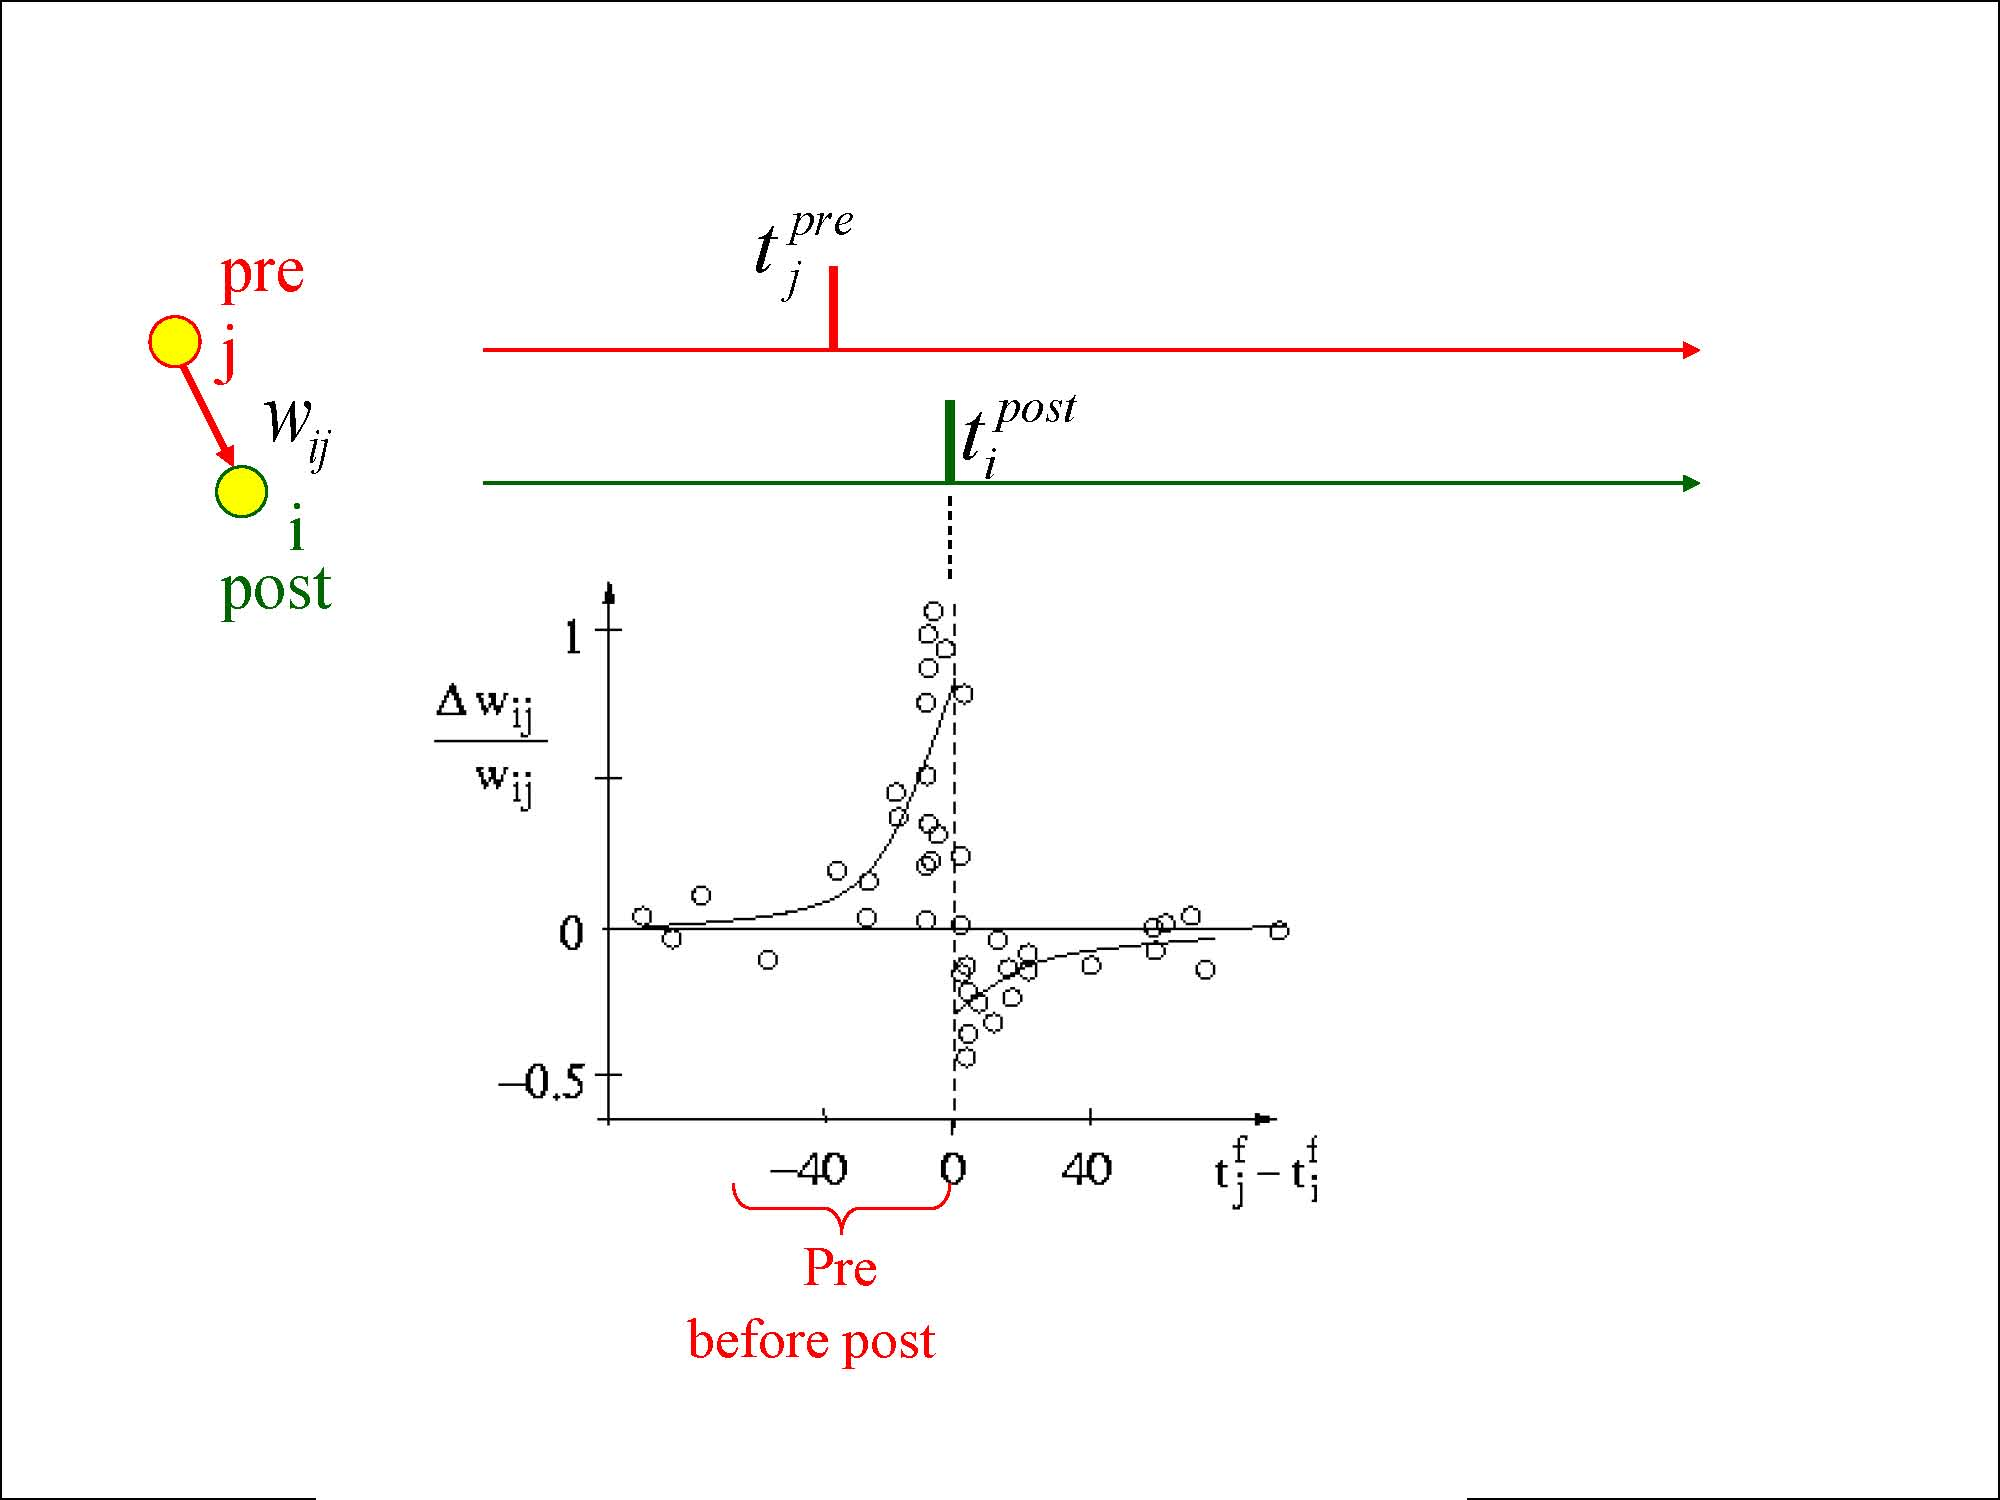
\includegraphics[width=0.8\textwidth]{pics_snn/fig_stdp_orig.jpg}
	\caption{Synaptic Time Dependant Plasticity~\cite{gerstner2014neuronal}.}
	\label{Fig:STDP}
\end{figure}
%One of the key parameters of a neural network is the amount of influence each incoming spike has on a neuron.
The influence each incoming spike has on a post-synaptic neuron is modelled by assigning a `weight' to each synapse;
tuning on the weight scales the impact of a spike
arriving via that synapse.
Many learning models simulate the changes in weights over long periods of time observed within the brain.
The exact rules by which these weights are adjusted is the subject of much active research though most promising approaches attempt to learn from the relative timing \cite{pfister2006triplets} or rate \cite{bienenstock1982theory} of spikes arriving at a neuron.
As well as adjusting weights, some learning rules can also form entirely new connections between previously unconnected
neurons \cite{bamford2010synaptic}.

\section{Simulating Networks of Spiking Neurons}
\label{sec:snn_sim}
\subsection{Software Simulators}
clock driven

event driven

hybrid simulators Brian, Nest and Neuron

PyNN
\subsection{Neuromorphic Hardware}
Table from Steve
\subsection{Neuromorphic Standing-alone Systems}
Papers listed.
Vision and Auditory
\label{sec:morph}

